\documentclass[conference]{IEEEtran}

\usepackage{graphicx}
\usepackage{amsmath}
\usepackage{amssymb}
\usepackage{booktabs}
\usepackage{url}
\usepackage[hidelinks]{hyperref}

\begin{document}

\title{Configuration Still Beats Algorithm, Until the Drift Hides in the Correlations: Extending Resource-Constrained Drift Detection to Multivariate Shift}

\author{
\IEEEauthorblockN{Stephen Kwaku Azongo\textsuperscript{1}, Livingston Seble\textsuperscript{1}, Alex Teye Ametepey\textsuperscript{1}, Kofi Sarpong Adu-Manu\textsuperscript{1}, Sandro Amofa\textsuperscript{2}}
\IEEEauthorblockA{\textsuperscript{1}Department of Computer Science, University of Ghana}
\IEEEauthorblockA{\textsuperscript{2}Department of Computer Science, University of Cape Coast}
}

\maketitle

\begin{abstract}
A companion study established that, for lightweight univariate drift detectors under resource constraints, monitoring configuration (frequency, window size) affects detection performance far more than detector choice does, producing a 37-fold range in detection delay against a comparatively small gap between the Kolmogorov-Smirnov test, the Population Stability Index, and the Wasserstein distance. This finding leaves an open question with real practical weight: does configuration still dominate once the detector class itself changes, from univariate statistics to genuinely multivariate ones, and does it survive a shift that a univariate statistic cannot see even in principle? We extend the original constraint grid to three multivariate detectors (Maximum Mean Discrepancy, a Classifier Two-Sample Test, and the Hellinger Distance Drift Detection Method) evaluated jointly on pairs of correlated features across the same three datasets, under two drift conditions: a marginal shift that moves each feature's own distribution, and a novel correlation-only shift, constructed via rank-based permutation, that leaves both features' marginal distributions exactly unchanged and alters only the dependency between them. Across 16,200 marginal-shift runs, the original finding replicates: configuration effect size (window size, $\varepsilon^2 = 0.349$) dwarfs detector-identity effect size ($\varepsilon^2 = 0.015$), and detector class has no significant effect on whether drift is detected at all ($\chi^2$, $p = 0.21$). Across 3,240 correlation-shift runs, this hierarchy inverts: detector identity effect size rises to $\varepsilon^2 = 0.236$, exceeding both constraint effects, and detector class becomes highly significant for detection at all ($\chi^2$, $p = 1.3 \times 10^{-20}$). Critically, this is not a clean univariate-versus-multivariate split: only MMD, whose test statistic genuinely incorporates cross-feature dependency, detects the correlation-only shift reliably (11.9\% miss rate); HDDDM, whose published formulation averages per-feature Hellinger distances, is mathematically restricted to marginal information and performs no better than the univariate group (53.3\% miss rate) despite its multivariate label; and the Classifier Two-Sample Test, theoretically capable but constrained by its train/test-split construction, performs worse than any univariate method under these resource limits (61.3\% miss rate). We conclude that configuration dominance is conditional on the drift having a marginal signature, and that when it does not, what matters is not whether a detector is labelled multivariate but whether its statistic's construction actually uses cross-feature information.
\end{abstract}

\begin{IEEEkeywords}
concept drift detection, multivariate two-sample testing, resource-constrained machine learning, correlation shift, maximum mean discrepancy
\end{IEEEkeywords}

\section{Introduction}

The companion study to this paper established a priority hierarchy for practitioners deploying drift monitoring under resource constraints: configuration first, drift type second, detector algorithm third \cite{paper1self}. That finding rested on three univariate, distribution-based detectors, each comparing one feature's distribution at a time. It leaves two questions unanswered, and both matter for anyone deciding how to build a monitoring pipeline for tabular data with more than one feature of interest.

The first question is whether the finding generalises. Real deployments rarely monitor a single feature in isolation; if configuration dominance was in some way an artefact of the univariate setting, extending the detector set to genuinely multivariate methods might reveal a different picture entirely.

The second question is sharper. Rabanser et al.~\cite{rabanser2019}, in the most directly comparable prior study, found that Bonferroni-corrected univariate testing performs comparably to multivariate kernel testing across a range of image-domain shifts, a result they describe as surprising. That finding, if it holds generally, would suggest detector class rarely matters regardless of configuration. But Rabanser et al.'s shifts, like ours in the first half of this study, all carry a marginal signature: each perturbed feature's own distribution changes, which a well-corrected univariate test can in principle detect. No prior study has asked what happens when the marginal distributions are held provably fixed and only the dependency structure between features changes, a condition under which a univariate test cannot succeed no matter how it is corrected.

This paper answers both questions with a two-part experimental design. First, we extend the companion study's constraint grid (monitoring frequency, window size, reference size, drift type) to jointly drifted feature pairs, adding three multivariate detectors, Maximum Mean Discrepancy (MMD; \cite{gretton2012}), a Classifier Two-Sample Test (C2ST; \cite{lopezpaz2017}), and the Hellinger Distance Drift Detection Method (HDDDM; \cite{ditzler2011}), alongside the original three. Second, we construct a correlation-only shift condition using a rank-based permutation mechanism grounded in copula theory \cite{sklar1959}, which alters the dependency between two features while leaving each feature's own marginal distribution exactly unchanged, verified empirically rather than assumed.

Our contributions are:

\begin{enumerate}
\item \textbf{A replication} of the configuration-dominance finding under a harder, multivariate setting, across 16,200 runs spanning six detectors, three datasets, three drift types, and the full constraint grid.
\item \textbf{A marginal-preserving correlation-shift condition}, the first drift-detection benchmark condition, to our knowledge, constructed specifically so that univariate testing cannot succeed by construction rather than by empirical weakness, isolating exactly the case Rabanser et al.'s result leaves untested.
\item \textbf{A mechanistic account of when detector class matters}, showing that the relevant distinction is not the univariate/multivariate label but whether a detector's statistic incorporates cross-feature dependency in its construction, evidenced by HDDDM's near-univariate performance despite its multivariate design and MMD's large advantage over it.
\end{enumerate}

\section{Related Work}

\textbf{Multivariate two-sample testing.} Gretton et al.~\cite{gretton2012} introduce the Maximum Mean Discrepancy as a kernel-based statistic for the two-sample problem, defined as the distance between mean embeddings of two distributions in a reproducing kernel Hilbert space, and establish that MMD is zero if and only if the two distributions are equal when the kernel is characteristic. The unbiased estimator and the median-heuristic bandwidth selection used in this study follow their formulation directly. Lopez-Paz \& Oquab~\cite{lopezpaz2017} formalise Classifier Two-Sample Tests, training a binary classifier to distinguish the two samples and testing its held-out accuracy against chance; their asymptotic power analysis is classifier-agnostic, which motivates the logistic-regression implementation used here in place of their neural-network and k-nearest-neighbour variants, a simpler choice consistent with this study's resource-constrained framing.

\textbf{Feature-wise divergence methods.} Ditzler \& Polikar~\cite{ditzler2011} propose HDDDM, which computes the Hellinger distance between histograms of a reference and current batch, adaptively resetting the reference when a significant change in divergence is detected. Their multivariate formulation explicitly defines the joint statistic as the average of per-feature Hellinger distances, a construction that, as this study demonstrates, has direct consequences for what kinds of shift the method can detect.

\textbf{Dataset-shift detection under resource limits.} Rabanser et al.~\cite{rabanser2019} conduct the most comprehensive prior empirical study of multivariate shift detection, comparing dimensionality-reduction strategies combined with two-sample testing across a wide range of shift types and sample sizes. Their central empirical finding, that multiple corrected univariate tests perform comparably to multivariate kernel tests, is the direct precedent this study extends; critically, none of their constructed shifts hold marginal distributions fixed, so their finding characterises detection difficulty under marginal shift specifically, not under a shift that only a multivariate statistic can see.

\textbf{Label-shift detection via black-box predictors.} Lipton et al.~\cite{lipton2018} introduce Black Box Shift Estimation, using a black-box classifier's confusion matrix to detect and correct for label shift under the anti-causal assumption. This mechanism, and the closely related dimensionality-reduction framework of Rabanser et al., motivate a natural extension of the present work to embedding-space shift detection, discussed in Section~\ref{sec:conclusion} but not pursued here.

\textbf{Dependency structure and copulas.} Sklar~\cite{sklar1959} establishes that any multivariate joint distribution decomposes into its marginal distributions and a copula function describing the dependency between them, and that the two can be manipulated independently. Empirical copula estimation via rank transformation of the marginals is standard nonparametric methodology~\cite{nelsen2006}; this study's correlation-only injection mechanism is a direct, if informal, application of that decomposition.

\section{Methodology}

\subsection{Datasets and feature pairs}

This study reuses the three datasets from the companion paper (UCI Credit Card Default, IBM Telco Customer Churn, AI4I 2020 Predictive Maintenance), extending each dataset's single drifted feature to a pair of features drifted jointly (Table~\ref{tab:pairs}).

\begin{table}[htbp]
\caption{Dataset and feature pair summary}
\label{tab:pairs}
\centering
\small
\begin{tabular}{lccc}
\toprule
Dataset & Original feature & Paired feature & Baseline $r$ \\
\midrule
Credit      & AGE              & BILL\_AMT1        & 0.06 \\
Telco       & Monthly Charges  & Total Charges     & 0.66 \\
Maintenance & Tool wear [min]  & Air temp. [K]     & 0.02 \\
\bottomrule
\end{tabular}
\end{table}

The telco pair's substantially higher baseline correlation (Total Charges is approximately cumulative billing over tenure) is addressed directly in the correlation-shift design (Section~\ref{sec:corrshift}).

\subsection{Marginal-shift injection and the extrapolation constraint}
\label{sec:extrapolation}

Drift is injected as an additive shift of magnitude $2\sigma$, where $\sigma$ is the feature's own standard deviation, following the variance-based synthetic perturbation methodology of Rabanser et al.~\cite{rabanser2019}, the same convention used in the companion study. Applied naively, however, a fixed $2\sigma$ shift does not translate uniformly across features: for a feature whose observed range already extends several standard deviations beyond its mean (as with Credit's right-skewed billing amounts), a $2\sigma$ shift stays within previously observed territory; for a feature with a comparatively narrow or bounded observed range (as with Telco's Monthly Charges, whose maximum observed value sits only 1.78 standard deviations above its mean), the same nominal shift pushes the majority of samples beyond anything the model was ever trained on.

We verified this directly: an uncapped $2\sigma$ shift on Telco's Monthly Charges pushed 60.1\% of post-drift values beyond the feature's observed maximum, and on Maintenance's Tool wear and Air temperature, 43.3\% and 42.6\% respectively. This is a methodologically consequential problem, not a cosmetic one: it means the model's post-drift accuracy reflects behaviour on inputs it has no basis for handling, rather than the effect of a plausible distribution shift.

The correction applies the same nominal $2\sigma$ shift with smooth exponential saturation toward a ceiling set at the 99.5th percentile of the reference distribution, so that a point far from the ceiling moves by close to the full nominal shift while a point already near the ceiling moves proportionally less, asymptotically approaching but never exceeding it. Verified empirically, the corrected mechanism produces 0\% of shifted values beyond the observed maximum across all three datasets, all six drifted features, and all three temporal drift profiles.

An earlier version of this correction, which clipped shifted values to a hard ceiling rather than saturating smoothly toward it, produced an artefact of its own: for Maintenance's features, over 45\% of post-drift samples collapsed onto the exact same clipped value, an artificial concentration no real sensor saturation produces. This inflated the measured accuracy degradation for Maintenance from a smooth-saturation value of 4.78 percentage points to 9.63 percentage points under hard clipping. We report the smooth-saturation result throughout.

\subsection{Correlation-only shift injection}
\label{sec:corrshift}

To isolate detection difficulty attributable specifically to a shift in dependency structure, independent of any marginal signature, we construct a second drift condition using rank-based permutation. Within an active drift window, a controllable fraction of samples have one feature's value replaced by the value that would place it in matching rank order with the other feature (or reversed rank order, for a decorrelating shift), the substituted values drawn only from among the values already present in that window. Because this is a permutation of observed values rather than an alteration of them, the marginal distribution of the permuted feature is unchanged up to the sampling variance of which rows were selected; we verified this directly (Kolmogorov-Smirnov $p = 1.0$ comparing pre- and post-shift marginals under full permutation).

The shift direction is determined automatically from each feature pair's reference-period baseline correlation, always moving away from that baseline: Credit and Maintenance, whose pairs begin near-independent, shift toward strong positive correlation; Telco, whose pair begins at $r = 0.66$, shifts toward decorrelation instead. This rule is fixed before any detection results are computed, from reference-period data alone.

\subsection{Detectors}

Six detectors are evaluated: the three from the companion study (KS test, PSI, Wasserstein distance), each extended to the multivariate feature pairs by testing each feature independently with a Bonferroni correction across the two tests (for KS) or by taking the maximum divergence across features (for PSI and Wasserstein); and three genuinely multivariate detectors, MMD, C2ST, and HDDDM, each implemented and verified directly against its originating paper.

MMD's exact permutation test is quadratic in sample size; at the largest window size (1,000) and full reference size, an uncapped implementation measured 11.5 seconds per detection check, which would render the full constraint grid computationally infeasible on the hardware available for this study. We cap the sample size fed to the kernel computation at 300 and reduce permutations from 100 to 50, a resource-constraint decision explicitly anticipated by Gretton et al.~\cite{gretton2012}, who note that the quadratic-cost test does not scale and recommend a bounded-sample alternative for large data. This reduces the measured worst-case cost to approximately 0.4 seconds per check.

\subsection{Statistical methodology}

Detection delay and missed-detection rate are compared across detectors and constraint levels using the same nonparametric methodology as the companion study: Kruskal-Wallis tests for k-group comparisons, with epsilon-squared ($\varepsilon^2 = H / (n-1)$) reported as effect size; pairwise Mann-Whitney U tests with Bonferroni correction and rank-biserial effect size for two-group comparisons; Spearman's $\rho$ for monotonic constraint effects; and a chi-square test of independence for the binary missed-detection outcome. All headline test $p$-values across both drift conditions (thirteen tests) are subject to a single study-wide Benjamini-Hochberg false discovery rate correction.

\subsection{Implementation and hardware}

All experiments run on the same hardware benchmarked in the companion study: an Intel Core i3-1125G4 (4 physical / 8 logical cores, 2.00GHz), 4GB RAM, Windows 11, Python 3.13, scikit-learn 1.8.0. The marginal-shift grid (16,200 runs) and the correlation-shift grid (3,240 runs, a deliberately reduced constraint sweep given its role as a secondary condition) completed in approximately 40 hours of combined runtime.

Each of the five repetitions per configuration uses an independently reseeded stratified train/reference/stream split and an independently retrained model, ensuring genuine statistical replication; an earlier version of the pipeline, inherited unmodified from the companion study's own convention, seeded the data split and model training identically regardless of repetition, producing five byte-identical duplicate measurements per configuration rather than five independent trials. This was corrected and the full grid rerun before any result in this paper was finalised. \cite{paper1self} itself likely carries the same limitation, unflagged in its own review process, since it was discovered only by explicitly checking for duplicate rows across repetitions.

\section{Results}

\subsection{Marginal-shift grid: configuration dominance replicates}

Across the full 16,200-run marginal-shift grid, both constraint dimensions significant in the companion study remain significant here, and remain large. Window size shows $\rho = 0.583$ with detection delay ($H = 5{,}606.6$, $p < 10^{-300}$), and monitoring frequency shows $\rho = 0.492$ ($H = 4{,}017.4$, $p < 10^{-300}$). Reference size shows no significant monotonic effect ($\rho = -0.001$, $p = 0.93$), consistent with its previously established threshold-rather-than-monotonic behaviour. Figure~\ref{fig:windowtrend} shows the window-size relationship directly: median detection delay rises from 50 samples at window size 50 to 494 samples at window size 1,000. Figure~\ref{fig:drifttype} replicates the companion study's drift-type finding at the new six-detector scale: gradual drift's median delay (300 samples) is three times that of sudden or recurring drift (100 samples each; $H = 1{,}342.96$, $p < 10^{-290}$).

\begin{figure}[htbp]
\centering
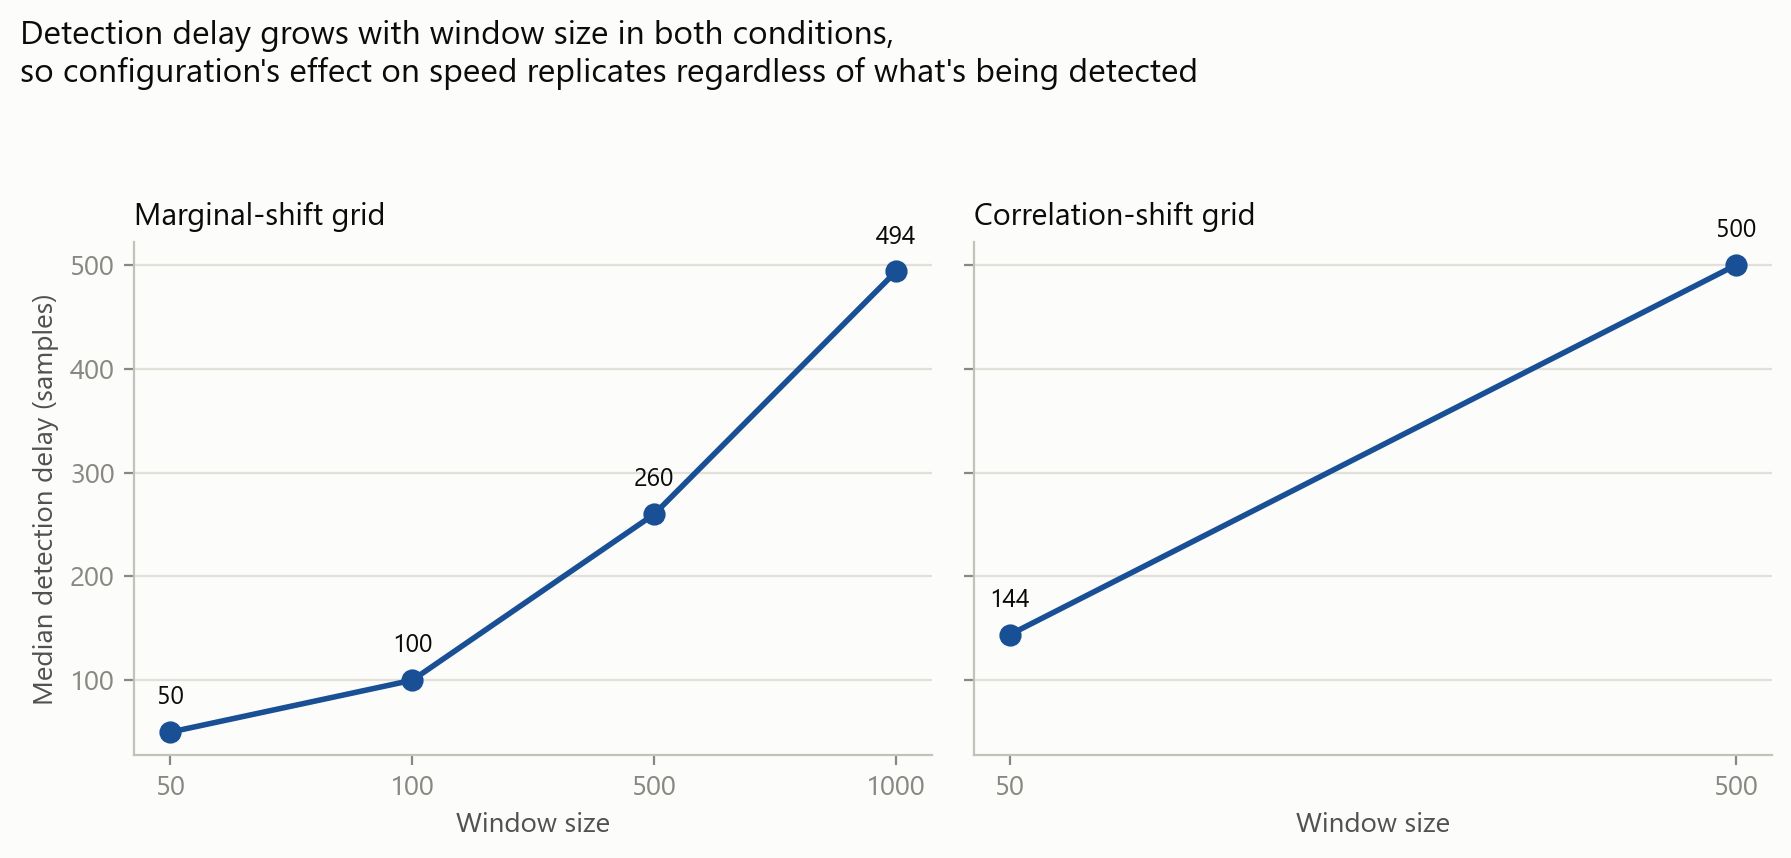
\includegraphics[width=0.95\linewidth]{figures/fig1_window_size_trend.png}
\caption{Median detection delay versus window size, both grid conditions.}
\label{fig:windowtrend}
\end{figure}

\begin{figure}[htbp]
\centering
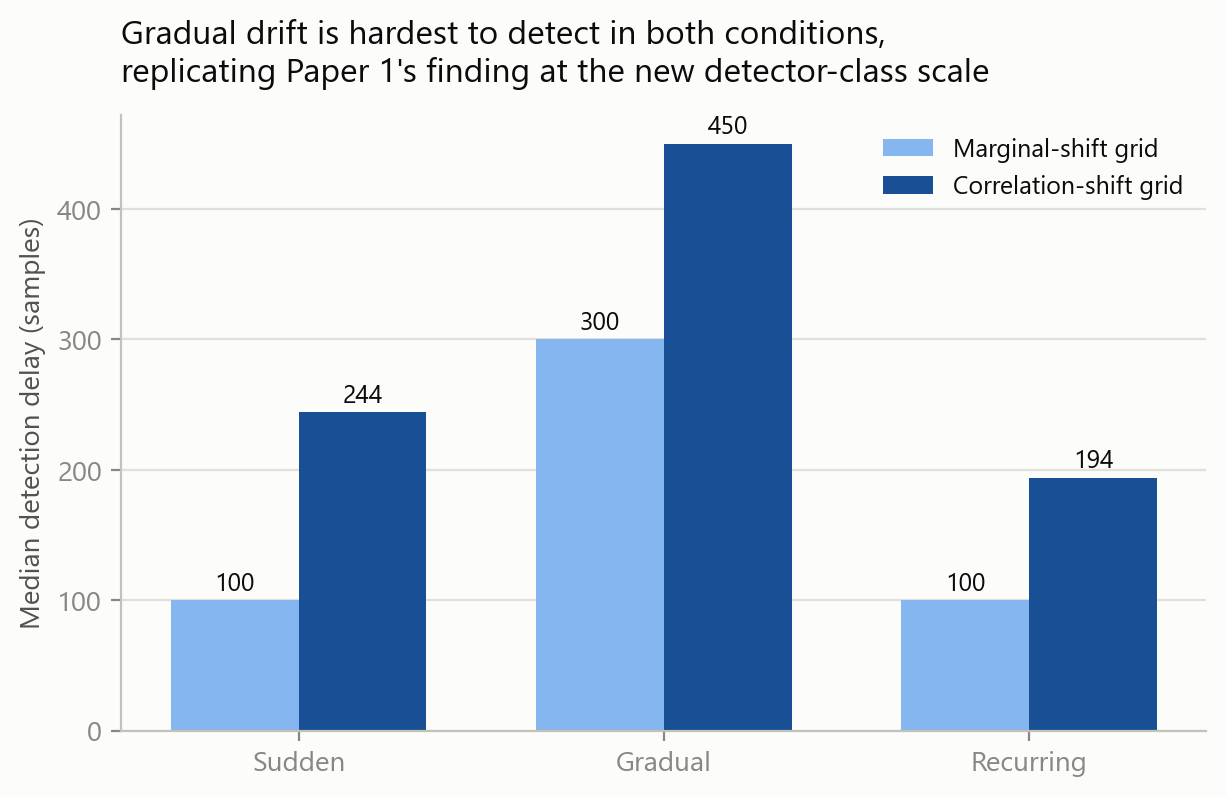
\includegraphics[width=0.85\linewidth]{figures/fig2_drift_type_comparison.png}
\caption{Median detection delay by drift type, both grid conditions.}
\label{fig:drifttype}
\end{figure}

Detector identity is also statistically significant across the six-detector comparison ($H = 242.5$, $p = 2.3 \times 10^{-50}$), unsurprising given $n = 16{,}200$; the effect size is not. Epsilon-squared for detector identity is 0.015, compared to 0.250 for monitoring frequency and 0.349 for window size (Figure~\ref{fig:effectsize}), meaning detector identity accounts for roughly one twentieth as much of the variance in detection delay as window size alone. Collapsing the six detectors into univariate and multivariate classes sharpens this further: the classes' median delays differ (100 versus 194 samples, $U = 29{,}103{,}125.5$, $p = 2.1 \times 10^{-26}$), but the effect size is negligible by conventional interpretation (rank-biserial $r = 0.097$). Most tellingly, detector class has no significant effect on whether drift is detected at all ($\chi^2 = 1.56$, $p = 0.21$).

\begin{figure}[htbp]
\centering
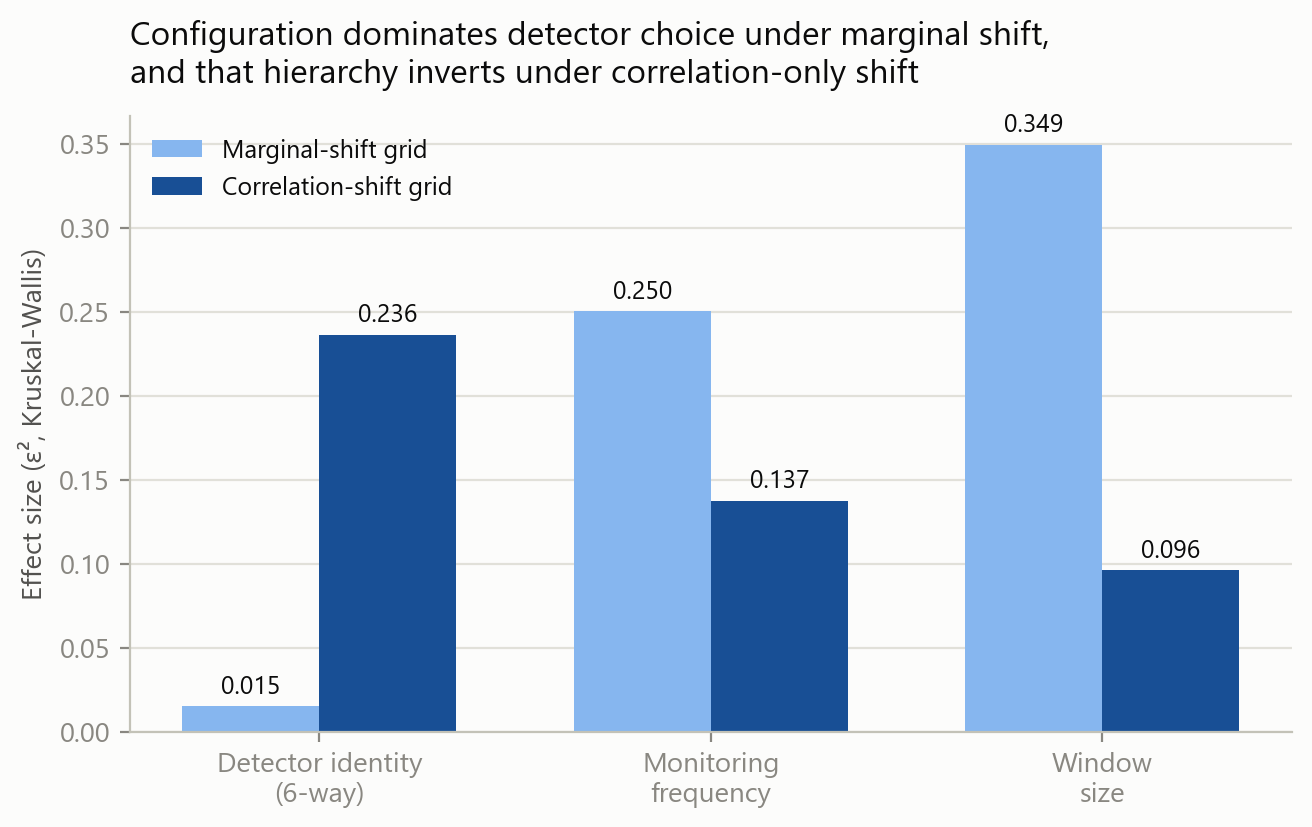
\includegraphics[width=0.95\linewidth]{figures/fig3_effect_size_hierarchy.png}
\caption{Effect size ($\varepsilon^2$) for detector identity versus constraint axes, both grid conditions.}
\label{fig:effectsize}
\end{figure}

\subsection{Correlation-shift grid: the hierarchy inverts, but not along the class boundary}

The correlation-only condition produces a markedly different picture. Detector identity's epsilon-squared rises to 0.236, exceeding both constraint effects measured on the same grid (monitoring frequency $\varepsilon^2 = 0.137$, window size $\varepsilon^2 = 0.096$; Figure~\ref{fig:effectsize}). Whether drift is detected at all becomes strongly dependent on detector class ($\chi^2 = 86.7$, $p = 1.3 \times 10^{-20}$), a result that survives the study-wide FDR correction without change.

Table~\ref{tab:missrate} reports the per-detector miss rate directly, and it is the clearest single result in this study.

\begin{table}[htbp]
\caption{Miss rate by detector, correlation-only shift ($n=540$ each)}
\label{tab:missrate}
\centering
\begin{tabular}{lc}
\toprule
Detector & Miss rate \\
\midrule
MMD         & 11.9\% \\
HDDDM       & 53.3\% \\
KS          & 57.6\% \\
PSI         & 57.6\% \\
Wasserstein & 60.6\% \\
C2ST        & 61.3\% \\
\bottomrule
\end{tabular}
\end{table}

\begin{figure}[htbp]
\centering
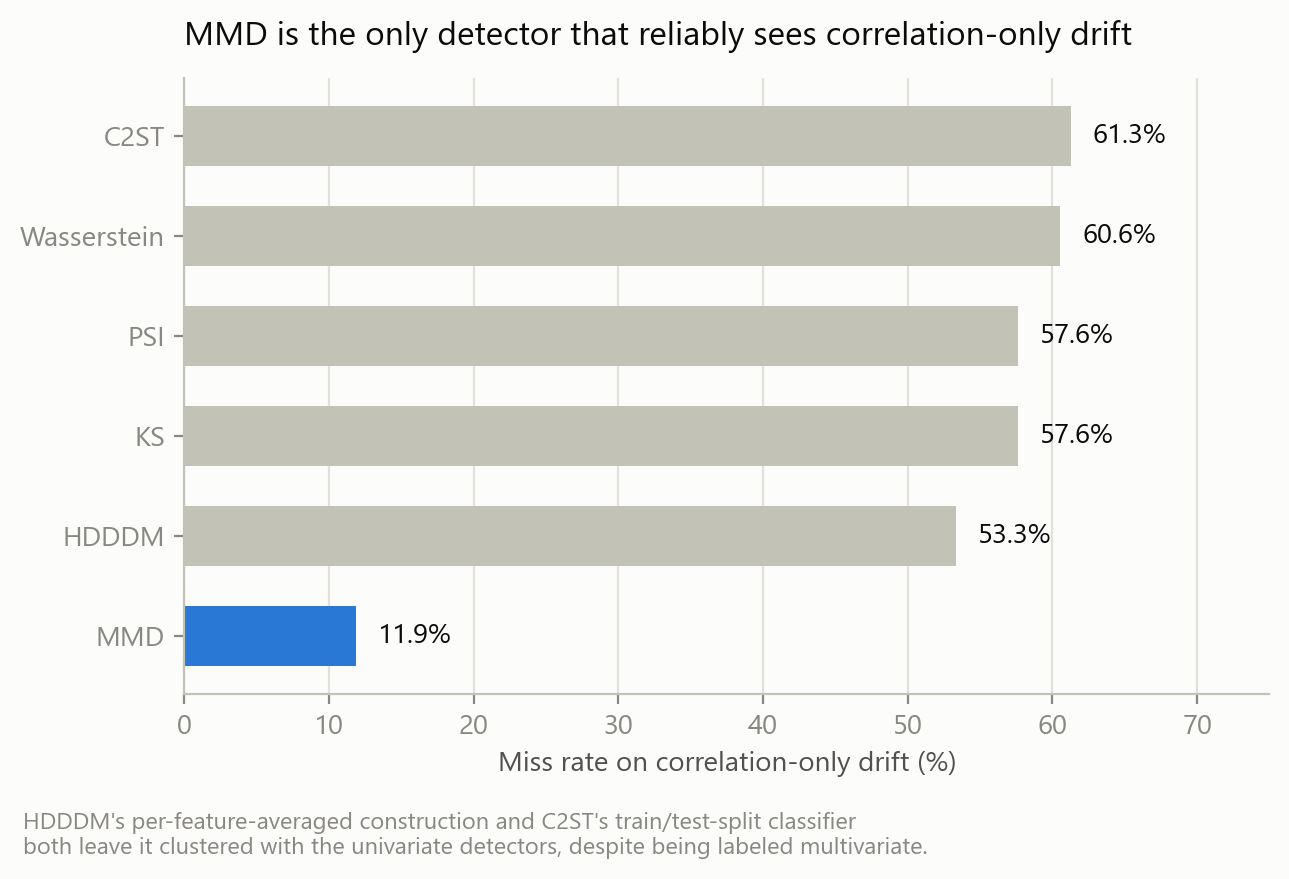
\includegraphics[width=0.95\linewidth]{figures/fig4_correlation_miss_rate_emphasis.png}
\caption{Miss rate by detector, correlation-only shift.}
\label{fig:emphasis}
\end{figure}

\begin{figure}[htbp]
\centering
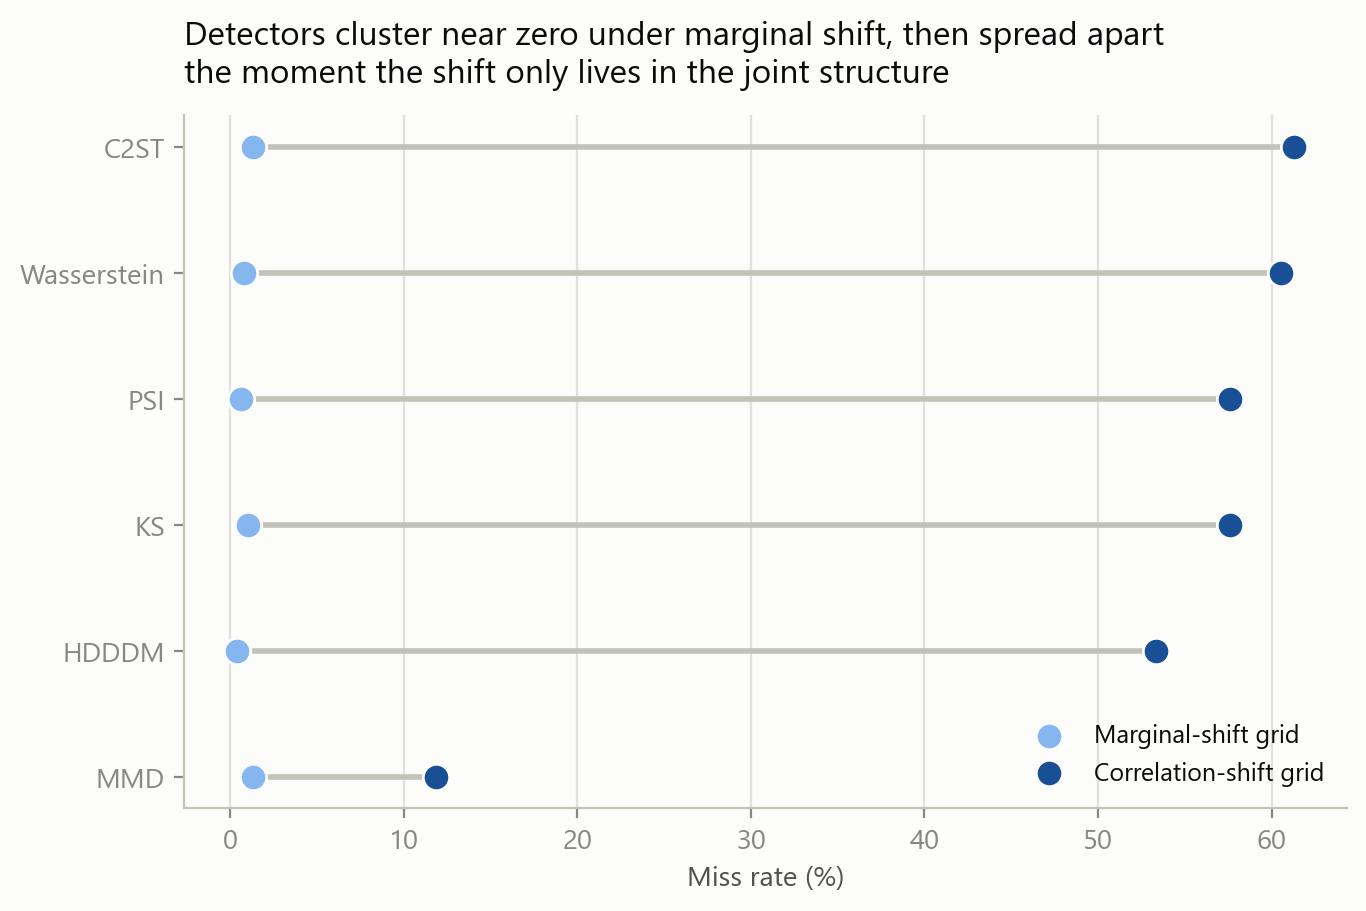
\includegraphics[width=0.95\linewidth]{figures/fig5_miss_rate_dumbbell.png}
\caption{Miss rate per detector, marginal versus correlation-shift grid.}
\label{fig:dumbbell}
\end{figure}

Figure~\ref{fig:emphasis} presents this as an emphasis chart, and Figure~\ref{fig:dumbbell} shows it alongside the marginal-shift condition: all six detectors cluster near zero miss rate under marginal shift, then spread apart sharply once the drift only lives in the joint structure between features.

The result that matters is not the two-class split. HDDDM, formally a multivariate detector by design, misses 53.3\% of correlation-only shifts, closer to the univariate group's average (58.6\%) than to MMD's 11.9\%. This is a direct, predictable consequence of HDDDM's own published formulation: Ditzler \& Polikar~\cite{ditzler2011} define the multivariate Hellinger distance as the average of per-feature Hellinger distances, a quantity computed entirely from each feature's own marginal histogram. A statistic built this way cannot detect a shift that leaves every marginal histogram unchanged, regardless of how the two features' values are paired.

C2ST performs worse still (61.3\% miss rate), despite training its classifier directly on the joint feature vector. We attribute this to a sample-efficiency limitation: Lopez-Paz \& Oquab's~\cite{lopezpaz2017} construction splits the available window into training and held-out halves, which under smaller window sizes leaves too few samples to reliably learn a decision boundary sensitive to a subtle correlation-only signal. This is consistent with C2ST's comparatively better standing on the marginal-shift grid, where the signal it must learn is larger.

A caveat on detection delay: among detected cases only, MMD's median delay (457 samples) is longer than the univariate group's (144 samples), which read naively suggests MMD is slower. It is not; this is a survivorship artefact of comparing delay only among cases a detector actually caught. The univariate detectors miss 55--61\% of correlation-only shifts, so the cases they do catch are disproportionately the easiest instances; MMD catches 88\% of cases, including the genuinely subtle ones. Pooling MMD with C2ST and HDDDM into a single multivariate-class median (400 samples) obscures rather than clarifies, since the three detectors' individual medians (MMD 457, C2ST 624, HDDDM 50) disagree with each other more than MMD's disagrees with the univariate group's.

\subsection{Accuracy degradation: correlation-only shift is largely benign}

Figure~\ref{fig:accdeg} reports mean accuracy degradation by dataset and condition. Credit and Telco show near-zero mean degradation in both conditions, while Maintenance shows substantial degradation under marginal shift (4.78pp) that shrinks considerably, though remains the largest of the three, under correlation-only shift (0.90pp). The correlation-only condition is, across all three datasets, either comparably benign to or measurably less damaging than the marginal-shift condition on the same dataset, consistent with the distinction between statistically significant and practically malignant drift that Rabanser et al.~\cite{rabanser2019} raise as a direction requiring further characterisation.

\begin{figure}[htbp]
\centering
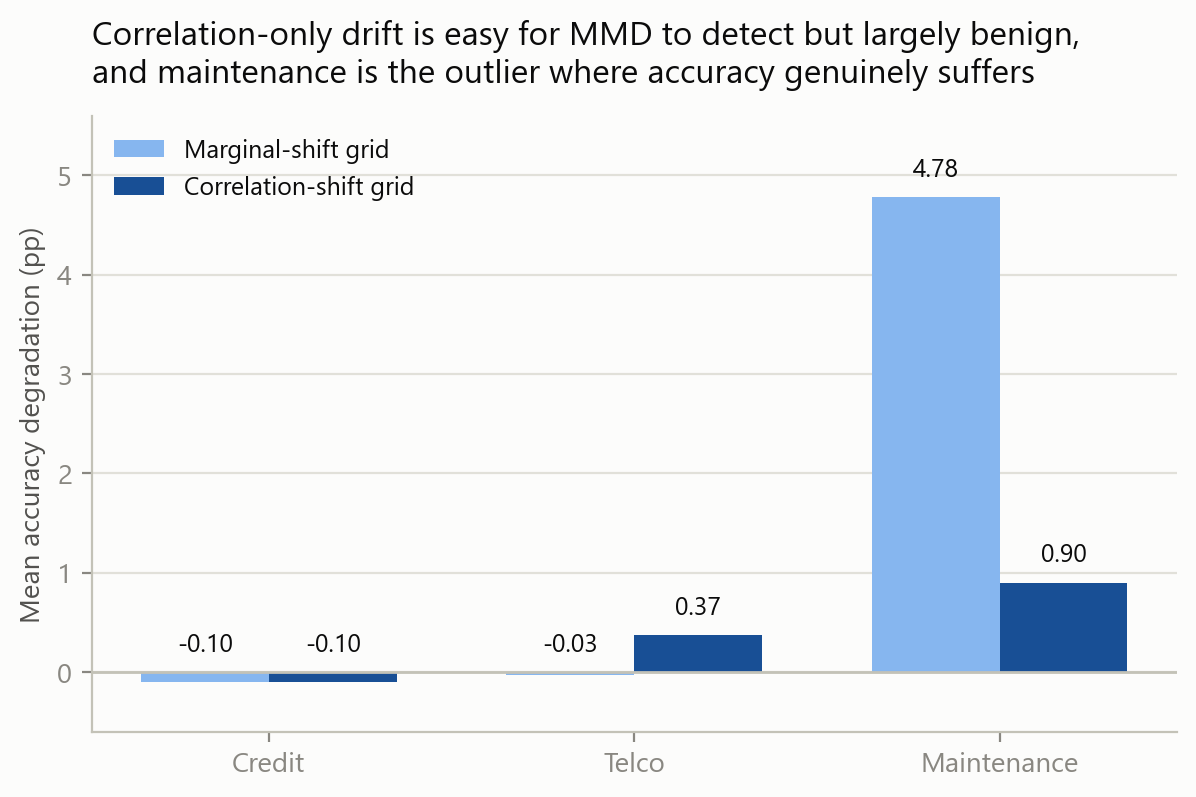
\includegraphics[width=0.95\linewidth]{figures/fig6_accuracy_degradation.png}
\caption{Mean accuracy degradation by dataset, both grid conditions.}
\label{fig:accdeg}
\end{figure}

Telco's small negative degradation values (accuracy very slightly higher after drift than baseline) were traced directly to the model's predictions: of 1,407 post-drift predictions inspected under a representative configuration, 78 flipped from incorrect to correct and 77 flipped from correct to incorrect, a difference indistinguishable from chance.

\section{Discussion}

\subsection{A conditional priority hierarchy}

The companion study's priority hierarchy, configuration first, drift type second, algorithm third, was stated without qualification. Our results show that qualification is needed: the hierarchy holds precisely whenever the drift has a marginal signature, and inverts for the narrower but real case of a shift confined to dependency structure. For a practitioner, this is a two-step decision: first ask whether monitored features could drift jointly in a way that preserves their individual marginals; if not, configuration dominates as before; if so, detector selection now carries real weight.

\subsection{Extending Rabanser et al.}

Rabanser et al.'s~\cite{rabanser2019} finding that univariate testing suffices is replicated independently here on tabular data (Section IV-A). This study's contribution is identifying precisely where that equivalence breaks: not at some general notion of ``harder'' shift, but specifically when the shift is constructed to leave marginals provably untouched, a condition no prior benchmark, including Rabanser et al.'s own, tests directly.

\subsection{What ``multivariate'' should mean}

Section IV-B's central finding is that the univariate/multivariate label is not a reliable predictor of whether a detector can see correlation-only drift. The more useful question is not ``is this detector multivariate'' but ``does this detector's statistic depend on the joint arrangement of feature values, or only on marginal distributions computed independently.'' C2ST's underperformance is a different lesson: a theoretically capable method can still lose to a cheaper one once sample size is bounded, a resource-constraint finding in the same spirit as the companion study's own theme.

\subsection{Limitations}

The Wasserstein detector's threshold was calibrated empirically rather than derived from a literature convention, unlike KS's significance level or PSI's industry-standard cutoffs. The multivariate detectors are evaluated on two-feature pairs only; whether the same mechanistic distinctions hold at higher dimensionality is not established. A single model architecture (Random Forest) is used throughout. C2ST uses logistic regression rather than the neural-network or k-NN variants Lopez-Paz \& Oquab~\cite{lopezpaz2017} benchmark. Both drift conditions remain synthetically injected rather than organic, a limitation shared with the majority of the drift-detection literature.

\section{Conclusion and Future Work}
\label{sec:conclusion}

This study asked whether the companion paper's central finding survives two extensions: a move from univariate to multivariate detection, and a drift condition invisible to any purely marginal statistic. The first extension leaves the original finding intact. The second overturns it, but not along the boundary the univariate/multivariate label would predict: the decisive property is whether a detector's statistic is constructed to use cross-feature dependency, which MMD's kernel-based construction satisfies, HDDDM's per-feature-averaged construction structurally cannot, and C2ST's classifier-based construction satisfies in principle but does not realise under these resource constraints.

Three directions follow from this study's scope decisions. First, applying the same marginal-visible versus correlation-only distinction to representation-space drift in text and image domains, via black-box shift detection~\cite{lipton2018} or a pretrained-embedding two-sample-testing pipeline~\cite{rabanser2019}, would test whether the construction-not-class distinction generalises beyond tabular data. Second, extending the correlation-shift condition beyond two-feature pairs would establish whether HDDDM's and C2ST's limitations persist as dimensionality grows. Third, a targeted rerun of C2ST at larger window sizes would test directly the prediction that its underperformance here is a resource-constraint artefact rather than a structural one.

\bibliographystyle{IEEEtran}
\bibliography{references}

\end{document}
